\section{Bevægelsesanalyse} \label{bevaegelse}
\textit{Følgende afsnit indeholder en bevægelsesanalyse af gang, løb og cykling. Dette udarbejdes med henblik på at finde karakteristika for de tre aktivitetsformer i forbindelse med detektering af aktiviteterne. Der vil derfor afslutningsvist være en sammenligning af karakteristika for de tre aktivitetsformer.}

\subsection{Gang}
Gang er en fysisk aktivitet, som er kendetegnet ved altid at have mindst en fod i jorden. Aktiviteten betegnes som en cyklus, der ses på \figref{fig:gang_cyklus}. Bevægelserne er identiske for højre og venstre ben men er forskudt med en halv cyklus i forhold til hinanden, hvorfor bevægelsen kun beskrives for højre ben.~\citep{VaughanDavisOConnor1992,Whittle1990} 
\begin{figure}[H]
	\centering
	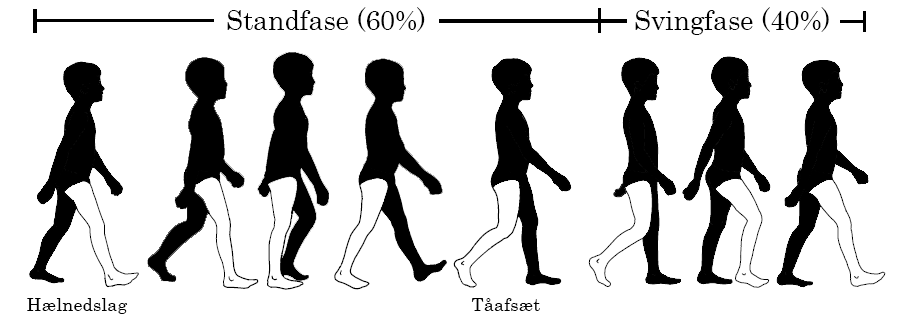
\includegraphics[scale=0.7]{figures/bProblemloesning/gang_cyklus.png}
	\caption{På figuren ses en gangcyklus, som er illustreret for højre ben, opdelt i henholdsvis en standfase og en svingfase. Standfasen udgør en større procentdel af den samlede cyklus end svingfasen. Ydermere indeholder standfasen cyklussens hælnedslag og tåafsæt.~\citep{VaughanDavisOConnor1992} (Modificeret)}
	\label{fig:gang_cyklus}
\end{figure}\vspace{-0.25cm}
Følgende beskrivelse tager udgangspunkt i \figref{fig:gang_cyklus}. En gangcyklus inddeles i to faser: standfasen og svingfasen. Standfasens varighed er cirka 60\% af en gangcyklus og påbegyndes, når den højre hæl opnår kontakt med underlaget. Efter dette placeres foden fladt på underlaget, da venstre fod her hæves over jorden. Herefter opnår begge fødder kontakt med underlaget, mens der opstår et hælslip for den højre fod. Standfasen afsluttes med en dorsalfleksion af anklen og dermed et afsæt fra tæerne på højre fod.~\citep{VaughanDavisOConnor1992,Whittle1990}  \newline 
Når højre fod samt højre ben er i svingfasen, udgør dette cirka 40\% af en gangcyklus. Svingfasen påbegyndes med en acceleration af foden og benet, når foden ikke længere har kontakt med underlaget i standfasen. Den højre fod svinges fremad lige under kroppen. Afsluttende for svingfasen er der en deacceleration. Denne fase sænker hastigheden af benets og fodens fremadgående bevægelse. Derved er kroppen klar til det kommende hælnedslag, som initierer standfasen.\fxnote{herefter gentages cyklussen}~\citep{VaughanDavisOConnor1992,Whittle1990}

De to faser er dermed i retningerne af henholdsvis x- og y-aksen. \Figref{fig:kraefter_akser} viser kraftpåvirkningen på begge akser, som forekommer ved et hælnedslag.  
\begin{figure}[H]
	\centering
	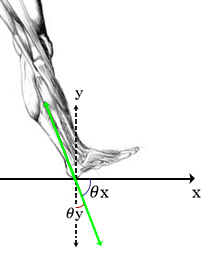
\includegraphics[scale=0.7]{figures/bProblemloesning/kraefter_akser.png}
	\caption{På figuren ses kraftpåvirkningerne for x- og y-aksen ved et hælnedslag. Den resulterende kraft ved hælnedslag er indikeret med en grøn pil. Denne har en mindre vinkel til y-aksen, hvormed kraftpåvirkningen i y-aksens retning er størst.}
	\label{fig:kraefter_akser}
\end{figure}\vspace{-0.25cm} 
\Figref{fig:kraefter_akser} illustrerer den resulterende krafts retning i forbindelse med et hælnedslag. Yderligere fremgår det, at vinklen mellem den resulterende kraft og y-aksen er mindre end vinklen mellem x-aksen og den resulterende kraft. Kraftpåvirkningen i forbindelse med et hælnedslag er altså størst i y-aksens retning og derfor mest karakteristisk.~\citep{Rueterbories2010,Serway2010,ClelandKikhia2013}

\subsection{Løb}
Løb er en fysisk aktivitet, som er kendetegnet ved, at maksimalt én fod rører jorden af gangen. Aktiviteten er en hurtigere version af gang og beskrives ligeledes som en cyklus men indeholder fire faser, som det ses på \figref{fig:loebecyklus}: standfasen, den første svævefase, svingfasen og den anden svævefase. \citep{Adelaar1986,Novacheck1998}
\begin{figure}[H]
	\centering
	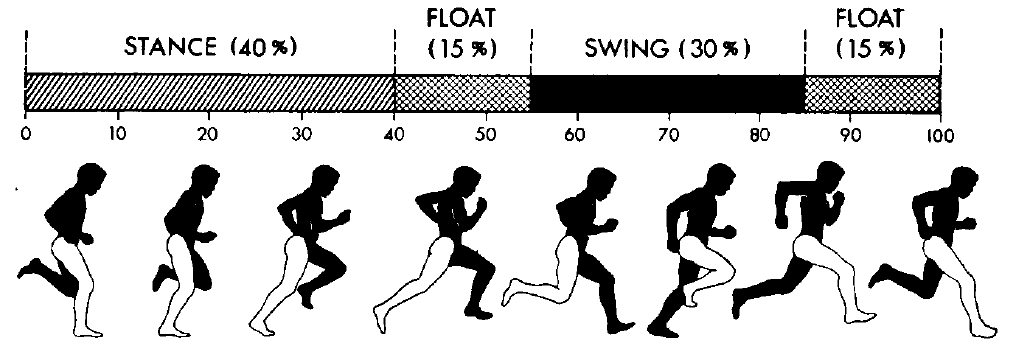
\includegraphics[scale=0.55]{figures/bProblemloesning/loeb_cyklus1.png}
	\caption{På figuren ses en løbecyklus opdelt i standfase, svingfase og to svævefaser. Standfasen udgør en større procentdel af cyklussen i forhold til svingfasen. Yderligere fremkommer svævefaser ved løb.~\citep{Adelaar1986} (Modificeret)}
	\label{fig:loebecyklus}
\end{figure}\vspace{-0.25cm}
Følgende beskrivelse tager udgangspunkt i \figref{fig:loebecyklus}. På samme vis som ved gangcyklussen begynder løbecyklussen, når højre hæl rammer jorden. Dette er begyndelsen af standfasen, som udgør 40\% af løbecyklussen. Herefter fortsætter foden til midtstand, hvor den er fladt placeret på jorden. Afslutningsvis udføres et accelererende afsæt med tæerne, som leder op til den næste fase, der er den første svævefase.~\citep{Adelaar1986,Novacheck1998} \newline 
De to svævefaser er identiske og udgør hver især 15\% af cyklussen. Disse er karakteriseret ved, at begge ben er løftet fra jorden. Svævefasen begynder idet, at tåafsættet har løftet foden fra jorden. Mellem de to svævefaser er svingfasen, som udgør 30\% af løbecyklussen. Denne fase indebærer, at højre fod og ben hæves og føres frem, hvorefter hælen igen isættes. Dette sker, mens den venstre fod udfører standfasen, hvorved højre fods svingfase er støttet af den venstre fod i jorden.~\citep{Adelaar1986,Novacheck1998} %Efter denne svævefase fase udføres anden svævefase før en ny cyklus kan påbegyndes. 

Ved løb er maksimalt én fod i kontakt med jorden ad gangen, hvilket resulterer i at der er et større stress på leddene ved løb i forhold til gang.~\citep{Adelaar1986} Dette suppleres af kraftpåvirkningen i de forskellige retninger under både gang og løb, hvor faserne domineres forskelligt af kraftpåvirkning i x- og y-aksens retning. \newline 
Standfasens hælnedslag og tåafsæt under gang og løb  er særligt karakteristisk grundet sin kraftpåvirkning i y-aksens retning. Kraftpåvirkningen er dog større ved løb, da denne fase ikke er understøttet af venstre fod. Kraftpåvirkningen i x-aksens retning for standfasen er af mindre betydning, da foden sættes i jorden og løftes op igen.\fxnote{Denne er større ved løb end gang, da hæl-nedslaget, som det ses på \figref{fig:loebecyklus}, er mere skråt på/har en mindre vinkel i forhold til jordoverfladen.} Modsat har svingfasen under gang og løb størst kraftpåvirkning i x-aksens retning, da accelerationen fremad af knæ og fod påvirker x-aksen mere end y-aksen.~\citep{Rueterbories2010} 

\subsection{Cykling}
Cykling er en aktivitetsform, der udnytter kraftoverførslen mellem en person og en cykel. For at opnå en fremdrift af cyklen benytter brugeren hovedsageligt en statisk position af overkroppen, hvorimod de nedre lemmer udfører kraftudviklingen.~\citep{Springer2014} Kraftoverførslen forekommer ved, at brugeren belaster cyklens pedaler. De roterende bevægelser med de nedre ekstremiteter skaber en fremdrift i hele systemet. Bevægelserne er opdelt i to lige lange faser; en kraftudøvende- og en restituerende fase, hvilket fremgår af \figref{fig:cykel_cyklus}.
\begin{figure}[H]
	\centering
	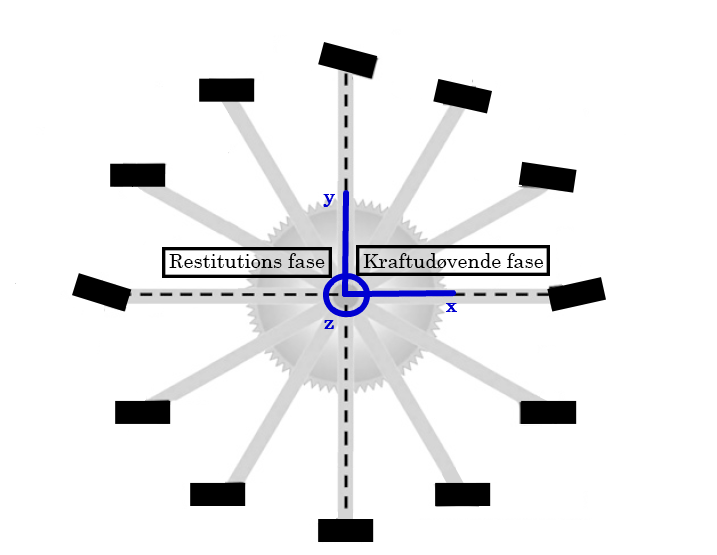
\includegraphics[scale=0.55]{figures/bProblemloesning/cykel_cyklus.png}
	\caption{På figuren ses cyklussen for cykling, som er opdelt to faser: en kraftudøvende- og en restituerende fase.~\citep{Springer2014} (Modificeret)}
	\label{fig:cykel_cyklus}
\end{figure}\vspace{-0.25cm}
Det fremgår af \figref{fig:cykel_cyklus}, at cykling er en bevægelse, som påvirker både x- og y-aksen. Der er dog tale om en cirkulær bevægelse om z-aksen. Idet cykling udføres i en cirkulær bevægelse, vil det være muligt at bestemme det antal grader, som benet har roteret om den pågældende akse. Derfor har en række studier beskrevet, at cykling med fordel kan detekteres af et gyroskop, som kan måle vinkelændringen af et bens bevægelse rundt om en akse. Dermed vil gyroskopets output for cykling være tilsvarende en sinussignal under ideelle forhold.~\citep{Cockcroft2011,Marin-PerianuMarin-Perianu2013} 

\subsection{Karakteristika for de tre aktivitetsformer}
En gangcyklus og løbecyklus er blandt andet karakteriseret ved at have en kraftpåvirkning i y-aksens retning ved hælnedslag og tåafsæt. Et eksempel på disse to kraftpåvirkninger i y-aksens retning kan ses under løb på \figref{fig:loeb_skolebog}. Signalet for gang vil til dels ligne dette signal dog med forskel på varigheden af henholdsvis stand- og svingfasen. Dette skyldes, at standfasen reduceres i varighed for løb i forhold til gang.
\begin{figure}[H]
	\centering
	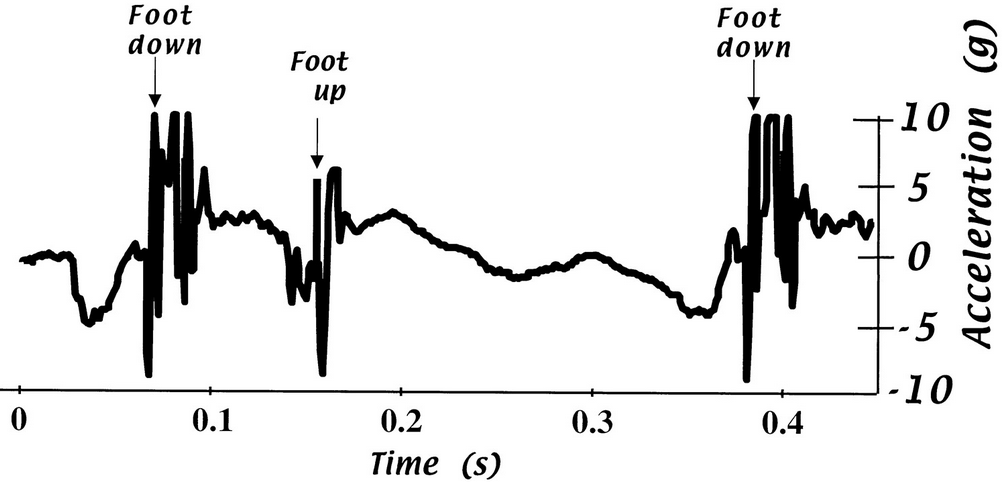
\includegraphics[scale=0.3]{figures/bProblemloesning/loeb_skolebog.png}
	\caption{På figuren ses et signal for løb optaget med et accelerometer, der er placeret på anklen. Accelerationen på y-aksen fremgår som funktion af tiden på x-aksen. En cyklus er angivet med den tilhørende stand- og svingfase, hvoraf de to svævefaser indgår i svingfasen. Ydermere er hælnedslag markeret med et blåt kryds, og et tåafsæt er markeret med en gul cirkel.~\citep{Strohrmann2011} (Modificeret)}
	\label{fig:loeb_skolebog}
\end{figure}\vspace{-0.25cm}
En cykelcyklus har ikke nogen væsentlig acceleration i vertikal eller horisontal retning men derimod rotation om en akse. Måling med et gyroskop vil dermed repræsentere ændringerne i vinklen om aksen.~\citep{Cockcroft2011,Marin-PerianuMarin-Perianu2013} 
